%----------------------------------------------------------------------------------------
%
% A LaTeX-template for 1DV510. Modified and translated by Björn Lindenberg at LNU.
% Based on an original master thesis template created by Marcus Wilhelmsson at LNU.
%
%----------------------------------------------------------------------------------------

% Settings and document configuration

\documentclass[a4paper,12pt]{article} 
\usepackage[T1]{fontenc} 
\usepackage{times} 
\usepackage[swedish,english]{babel} 
\usepackage[utf8]{inputenc} 
\usepackage{dtk-logos} 
\usepackage{wallpaper} 
\usepackage[absolute]{textpos} 
\usepackage[top=2cm, bottom=2.5cm, left=3cm, right=3cm]{geometry} 
\usepackage[parfill]{parskip} 
\usepackage{csquotes} 
\usepackage{float} 
\usepackage{lipsum} % Used for dummy text. Can be removed.
\usepackage{listings, color}
\lstdefinestyle{Asm}{
  belowcaptionskip=1\baselineskip,
  breaklines=true,
  frame=L,
  xleftmargin=\parindent,
  language=[x86masm]Assembler,
  showstringspaces=false,
  basicstyle=\footnotesize\ttfamily,
  keywordstyle=\bfseries\color{purple!40!black},
  commentstyle=\itshape\color{green!40!black},
  identifierstyle=\color{blue},
  stringstyle=\color{orange},
}

% Fontsizes for section headings.
\usepackage{sectsty} 
\sectionfont{\fontsize{14}{15}\selectfont}
\subsectionfont{\fontsize{12}{15}\selectfont}
\subsubsectionfont{\fontsize{12}{15}\selectfont}

%----------------------------------------------------------------------------------------
%	This part is used for the text box on the title page
%----------------------------------------------------------------------------------------
\newsavebox{\mybox}
\newlength{\mydepth}
\newlength{\myheight}

\newenvironment{sidebar}%
{\begin{lrbox}{\mybox}\begin{minipage}{\textwidth}}%
{\end{minipage}\end{lrbox}%
 \settodepth{\mydepth}{\usebox{\mybox}}%
 \settoheight{\myheight}{\usebox{\mybox}}%
 \addtolength{\myheight}{\mydepth}%
 \noindent\makebox[0pt]{\hspace{-20pt}\rule[-\mydepth]{1pt}{\myheight}}%
 \usebox{\mybox}}

%----------------------------------------------------------------------------------------
%	Title
%----------------------------------------------------------------------------------------
\newcommand\BackgroundPic{
    \put(-2,-3){
    
\includegraphics[keepaspectratio,scale=0.3]{img/lnu_etch.png} % Background image
    }
}
\newcommand\BackgroundPicLogo{
    \put(30,740){
    
\includegraphics[keepaspectratio,scale=0.10]{img/logo.png} % LNU logo
    }
}

\title{
\vspace{-8cm}
\begin{sidebar}
    \vspace{10cm}
    \normalfont \normalsize
    \huge Computer Technology I\\ % Main title
    \vspace{-1.3cm}
\end{sidebar}
\vspace{3cm}
\begin{flushleft}
    \huge Lab. 3 : Interrupts % Subtitle
     \small \\ \emph{}
\end{flushleft}
\null
\vfill
\begin{textblock}{5}(10,13)
\begin{flushright}
\begin{minipage}{\textwidth}
\begin{flushleft} \large
\emph{Author:}\textsc{Anas Kwefati}\\  % Author
\emph{Supervisor:}  \textsc{Anders Haggren} \\  % Author
\emph{Semester:} Autumn 2019\\ % Semester
\emph{Area:} Computer Science \\ % Area
\emph{Course code:} 1DT301 % Course
\end{flushleft}
\end{minipage}
\end{flushright}
\end{textblock}
}

\date{} % Empty date command. Use \today inside for today's date.
\author{} % Normally one would use this to define authors. However in this case the title command takes care of everything, so we leave the field empty to get rid of warnings. 

\begin{document}

\pagenumbering{gobble} % Turn off page numbering
\newgeometry{left=5cm}
\AddToShipoutPicture*{\BackgroundPic} % Adds the background image to the title page
\AddToShipoutPicture*{\BackgroundPicLogo} % Adds the logo to the title page
\maketitle % Prints the title
\restoregeometry
\clearpage

\pagenumbering{roman} % Roman page numbering for abstract page


\selectlanguage{english}

\newpage

\pagenumbering{gobble} % Turn off page numbering
\tableofcontents 

\newpage
\pagenumbering{arabic} % Turn on page numbering

%TASK1
\section{Task 1}
\lstset{style=Asm}

\begin{lstlisting}
;>>>>>>>>>>>>>>>>>>>>>>>>>>>>>>>>>>>>>>>>>>>>>>>>>>>>>>>>>>>
; 1DT301, Computer Technology I
; Date: 2016-09-15
; Author:
;	Anas Kwefati
;
; Lab number: 2
; Title: Interrupts
;
; Hardware: STK600, CPU ATmega2560
;
; Function: Write a program that turns ON and OFF when we push the button.
;The program must use interrupts
;
; Input ports: PORTD checks if we pressed the button
;
; Output ports: PORTB turns on/off the light (LEDs)
;
; Subroutines: If applicable.
; Included files: m2560def.inc
;
; Other information:
;
; Changes in program: (Description and date)
;<<<<<<<<<<<<<<<<<<<<<<<<<<<<<<<<<<<<<<<<<<<<<<<<<<<<<<<<<<<

.include "m2560def.inc"
;The term VECTOR means nothing more than that each interrupt has its specific address where it jumps to.
; The term TABLE means it is a list of jump instructions. This is a list of rjmp or jmp instructions, sorted by interrupt priority


.org 0x00 ;This is the location that the program will start executing from
rjmp start

.org INT0addr ;We are using INT0
rjmp interrupt ;we jump to interrupt when the External interrupt will occur

.org 0x72
start:
	; Initialize SP, Stack Pointer
	ldi r16, HIGH(RAMEND) ; R20 = high part of RAMEND address
	out SPH,r16 ; SPH = high part of RAMEND address
	ldi r16, low(RAMEND) ; R20 = low part of RAMEND address
	out SPL,r16 ; SPL = low part of RAMEND address



	;Main program initialization
	ldi r16, 0xFF ;
	out DDRB, r16 ; we set the DDRB as output


	ldi r17, 0b0000001 ;We set 0b00000001 to activate INT0
	out EIMSK, r17 ; Toggle external interrupt requests
	;EIMSK or External Interrupt Mask Register allows to set a bit to enable the related interrupt


	ldi r17, 0b00000010 ;We put 0b0000 0010 to r17
	;we do this to activate the interrupt during a falling edge
	sts EICRA, r17 ;EICRA allows us to define the type of signals
	;that activates the external interrupt

	sei ;enabling all interrupts


main_program:
nop ;we don't do anything
rjmp main_program ; we stay in the main_program until an external interrupt occurs



interrupt:
	com r16 ;we reverse the 0b1111 1111 to 0b0000 0000 like that we turn all light on
	out portB, r16 ;We output the value of r16 to the PORTB
reti ;return from interrupt instruction


\end{lstlisting}


\begin{figure}
\begin{center}
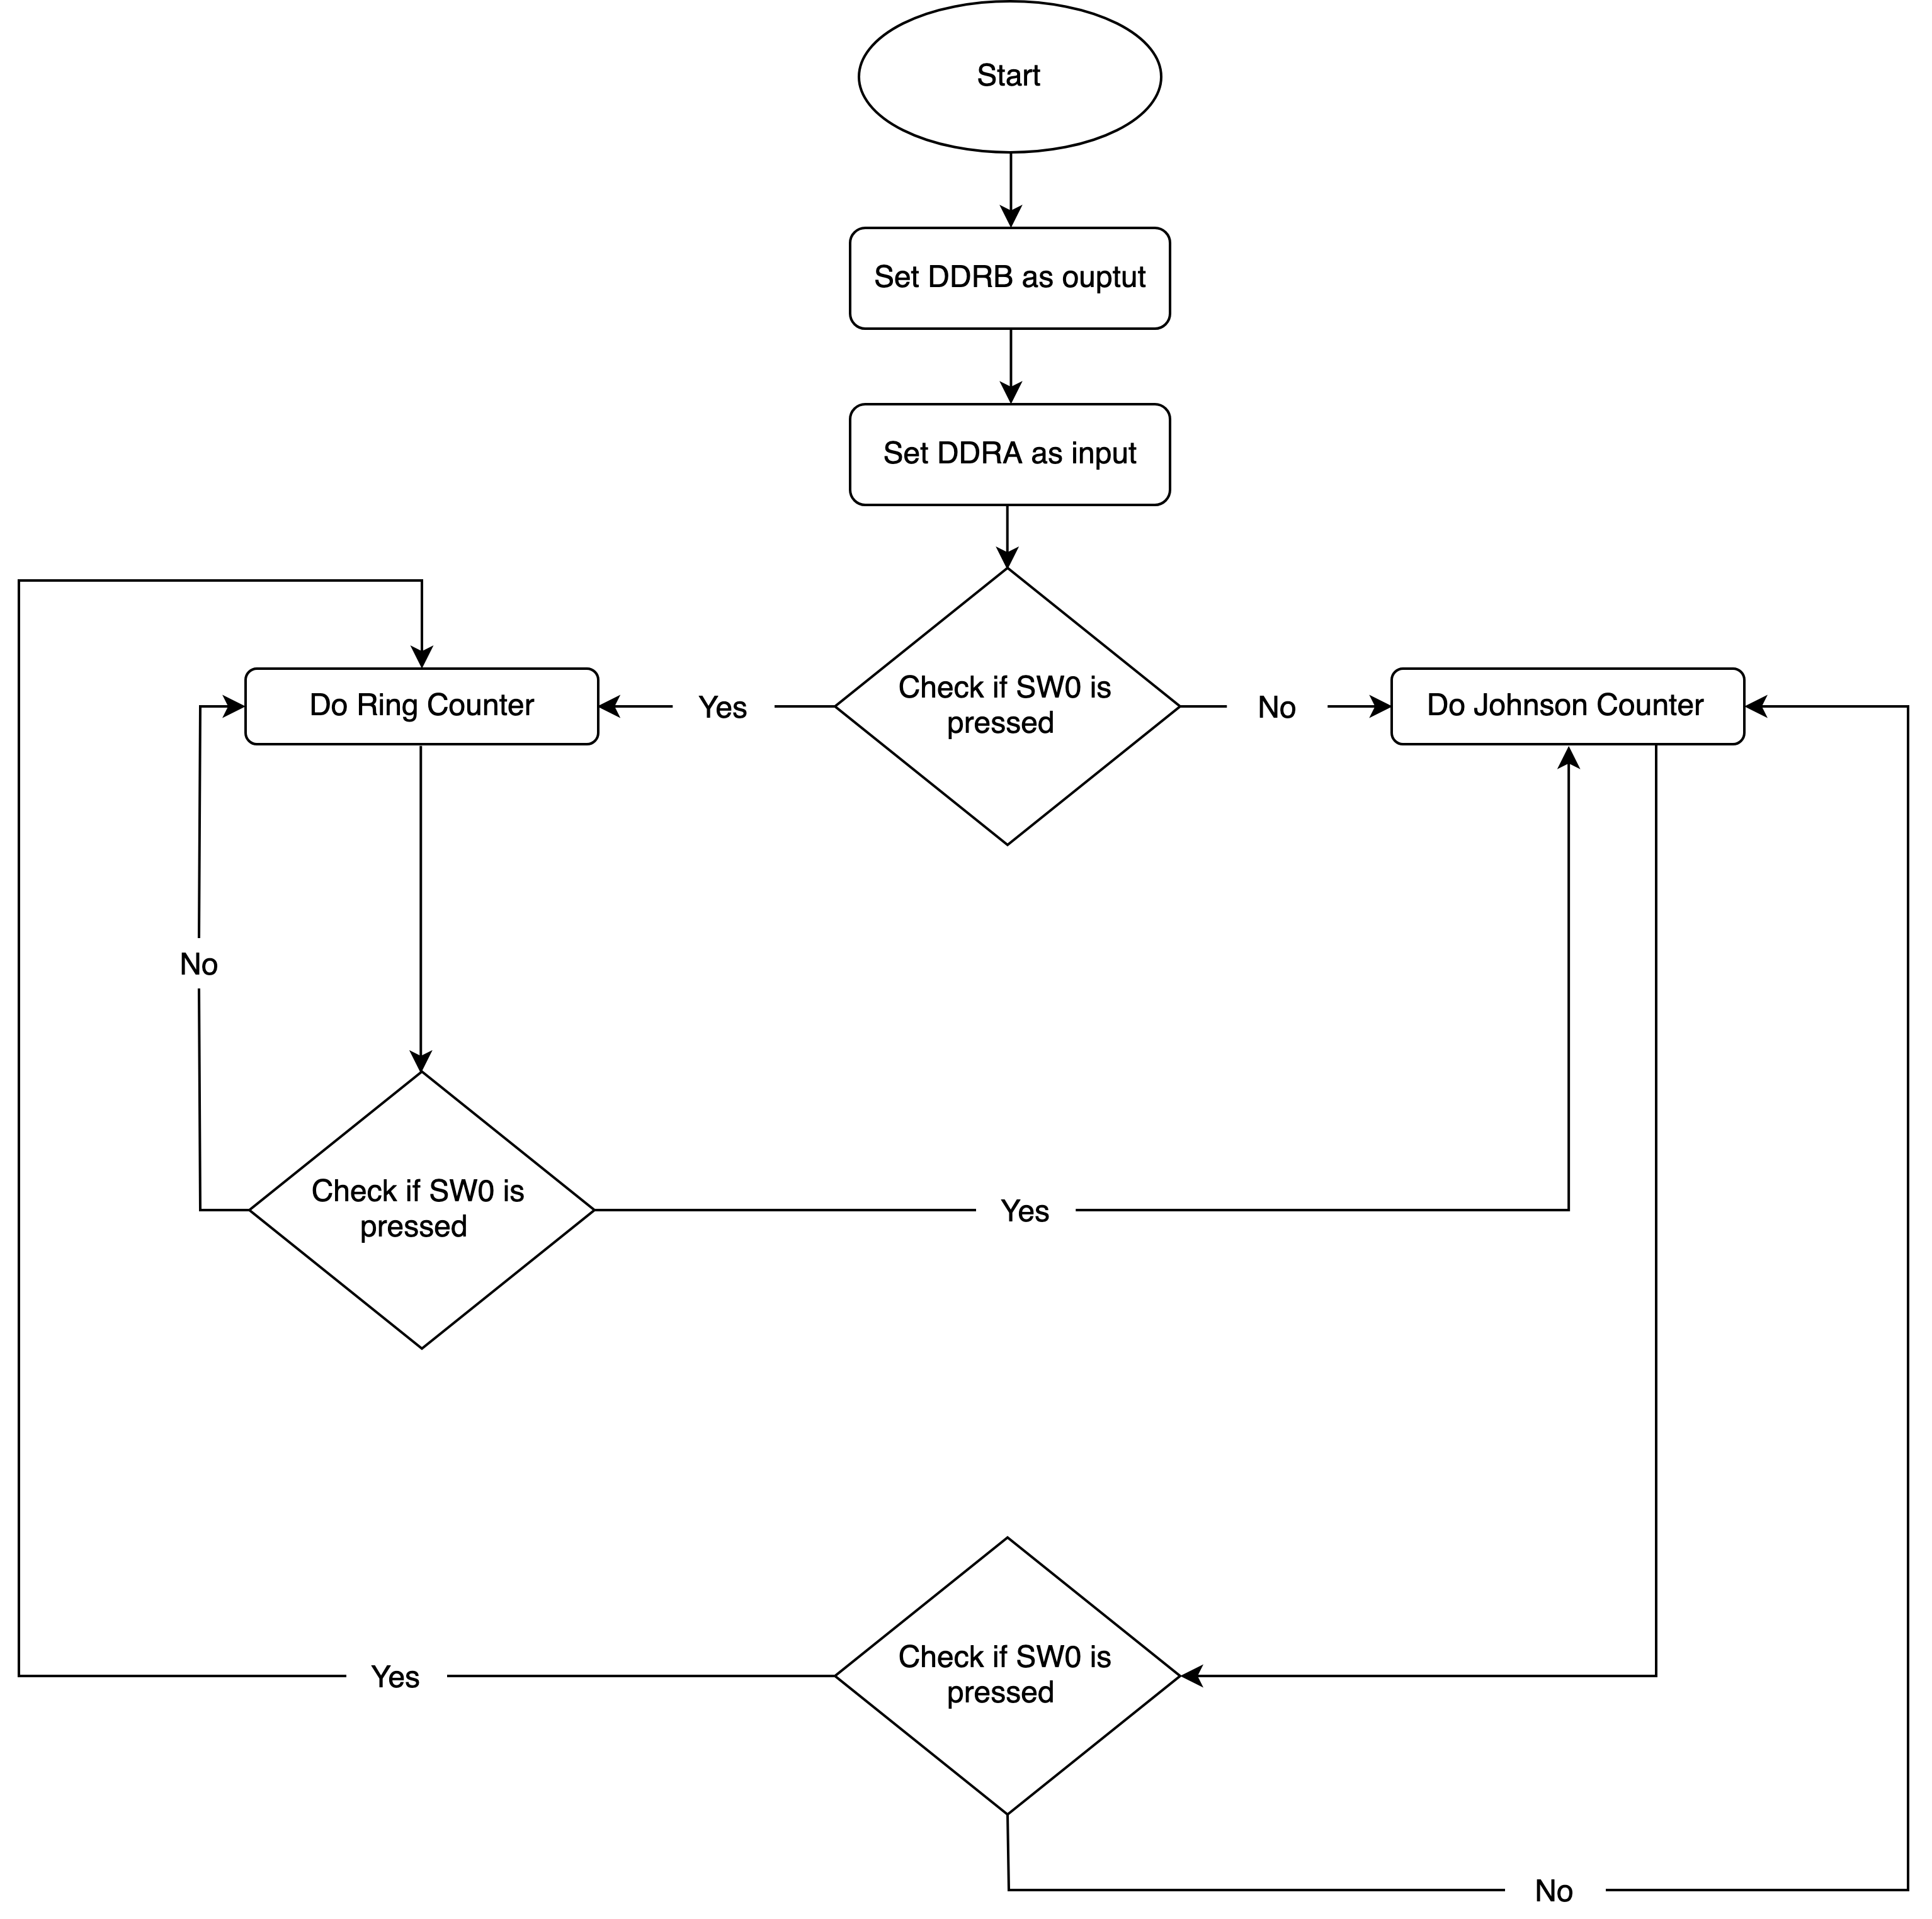
\includegraphics[width=\textwidth/1 ]{flowchart/task1_flowchart.png}
\end{center}
\caption{Task 1 flowchart}
\label{task1}
\end{figure}
\break


%TASK2
\section{Task 2}

\lstset{style=Asm}

\begin{lstlisting}
;>>>>>>>>>>>>>>>>>>>>>>>>>>>>>>>>>>>>>>>>>>>>>>>>>>>>>>>>>>>
; 1DT301, Computer Technology I
; Date: 2016-09-15
; Author:
;	Anas Kwefati
;
; Lab number: 3
; Title: Interrupts
;
; Hardware: STK600, CPU ATmega2560
;
; Function: The program switches between Ring Counter and Johnson counter
;We have to do this using interrupt when we push the button SW0 connected to PORTD
;
; Input ports: PORTD checks if we pressed the button
;
; Output ports: PORTB turns on/off the light (LEDs)
;
; Subroutines: If applicable.
; Included files: m2560def.inc
;
; Other information:
;
; Changes in program: (Description and date)
;<<<<<<<<<<<<<<<<<<<<<<<<<<<<<<<<<<<<<<<<<<<<<<<<<<<<<<<<<<<
.include "m2560def.inc"
;The term VECTOR means nothing more than that each interrupt has its specific address where it jumps to.
; The term TABLE means it is a list of jump instructions. This is a list of rjmp or jmp instructions, sorted by interrupt priority

.org 0x00 ;This is the location that the program will start executing from
rjmp start

.org INT0addr
rjmp interrupt

.org 0x72
start:
	; Initialize SP, Stack Pointer
	ldi r16, HIGH(RAMEND) ; R20 = high part of RAMEND address
	out SPH,r16 ; SPH = high part of RAMEND address
	ldi r16, low(RAMEND) ; R20 = low part of RAMEND address
	out SPL,r16 ; SPL = low part of RAMEND address



	;Main program initialization
	ldi r16, 0xFF ;
	out DDRB, r16 ; we set the DDRB as output


	ldi r17, 0b00000001 ;we set the corresponding bit number to enable the related interrupt here INT0
	out EIMSK, r17 ; Toggle external interrupt requests


	ldi r17, 0b00000010 ;We define the type of signals that activates the external interrupt , here we set it as falling edge to activate the interrupt
	sts EICRA, r17 ;we configure when to switch the external interrupt

	sei ;enabling all interrupts

ldi r25, 0b11111111 ;This will be changed thanks to the INT0 and com 25

ldi r16, 0b11111111 ;r16 will be used to compare with r25
ldi r22, 0b00000000 ;r22 will be used to compare with r25

main_program:
	cp r25, r16 ;we compare 0b1111 1111(r25) with 0b1111 1111 (r16)
	breq ring_counter ;if r25 == r16 go to ring_counter
rjmp main_program

;NORMAL RING_COUNTER
ring_counter:
	ldi r18, 0b11111110

	;WE COMPARE
	cp r25, r22 ;We compare r25 with 0b0000 0000 (r22)
	breq johnson_counter ;if r25 == r22 so we go to johnson_counter
	;if we press the SW0 and r25 becomes 0b0000 0000 because of the Int0
	;it will go to johnson_counter

ring_loop:
	out PORTB, r18 ;we put the value of r18 to PORTB which should turn on the light
	call Delay
	com r18
	LSL r18
	com r18

	;Check if everything is off if true then go to ring counter to make infinite loop
	ldi r24,0xFF
	cp r24, r18
	breq ring_counter

	;WE COMPARE
	cp r25, r22 ;We compare r25 with 0b0000 0000 (r22)
	breq johnson_counter ;if r25 == r22 so we go to johnson_counter
	;if we press the SW0 and r25 becomes 0b0000 0000 because of the Int0
	;it will go to johnson_counter

rjmp ring_loop

johnson_counter :
	ldi r19, 0b11111110 ;Turn on light at 0

	cp r25, r16 ;We compare r25 with 0b1111 1111(r16)
	breq ring_counter ;if r25 == r16 so it goes to ring_counter
	;if we press the SW0 and r25 becomes 0b1111 1111 because of the Int0
	;it will go to ring_counter

	ldi r22, 0x00 ;we load back 0b0000 0000 to r22 to not mess with the one of ring_counter

johnson_loop:
	out PORTB, r19
	LSL r19
	call Delay
	cp r19, r22
	breq johnson

	;WE COMPARE
	cp r25, r16 ;We compare r25 with 0b1111 1111(r16)
	breq ring_counter ;if r25 == r16 so it goes to ring_counter
	;if we press the SW0 and r25 becomes 0b1111 1111 because of the Int0
	;it will go to ring_counter

	rjmp johnson_loop


johnson :
	out PORTB, r22
	ldi r22, 0b11111111
	call Delay
	ldi r19,0b10000000

	more_john :
		out PORTB, r19
		ASR r19
		call Delay
		cp r19, r22
		breq johnson_counter

		;WE COMPARE
		cp r25, r16
		breq ring_counter

	rjmp more_john


 interrupt:
	com r25	;Whenever we press the button SW0, it takes the inverse.
	;So at first r25 is 0b1111 1111, then we press the button SW0
	;r25 becomes 0b0000 0000 and so on. By doing that we can compare it to r16 and r22
reti


Delay :
; Generated by delay loop calculator
; at http://www.bretmulvey.com/avrdelay.html

	ldi  r21, 5
    ldi  r23, 20
    ldi  r24, 175
L1: dec  r24
    brne L1
    dec  r23
    brne L1
    dec  r21
    brne L1
	ret

\end{lstlisting}
\break
\begin{figure}
\begin{center}
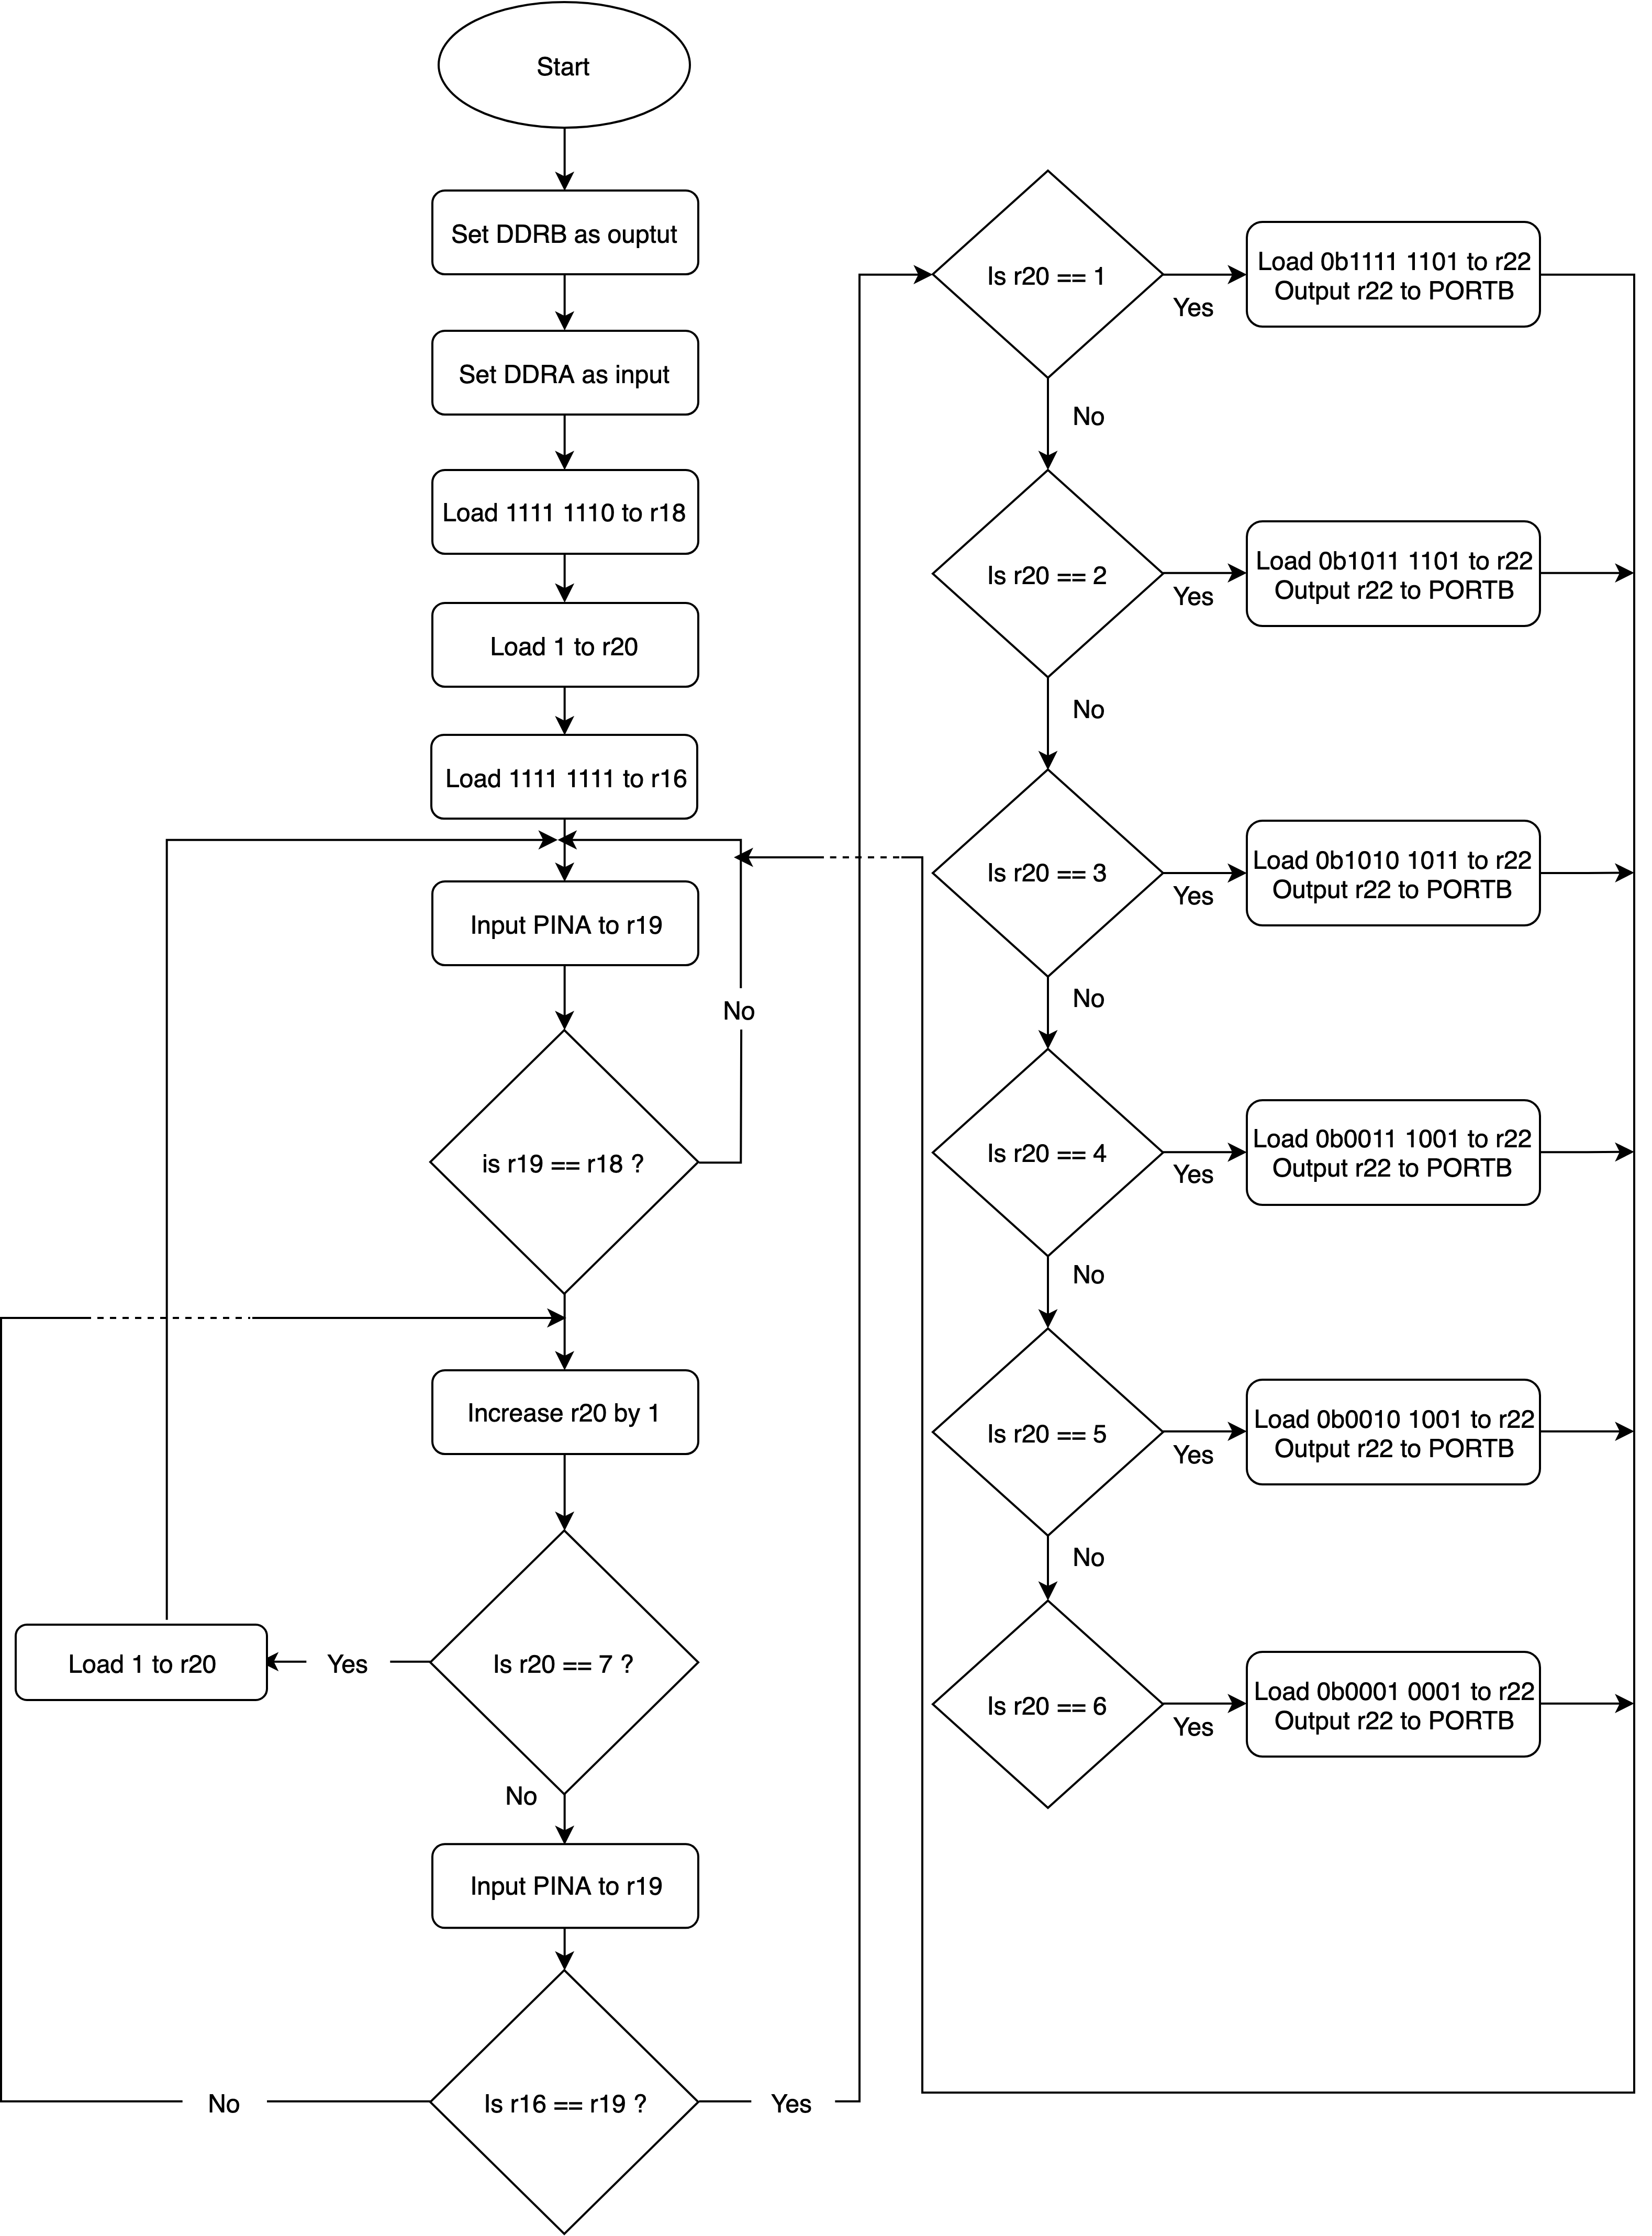
\includegraphics[width=\textwidth/1]{flowchart/task2_flowchart.png}
\end{center}
\caption{Task 2 flowchart}
\label{task2}
\end{figure}

\break


%TASK 3
\break
\section{Task 3}

\lstset{style=Asm}

\begin{lstlisting}
;>>>>>>>>>>>>>>>>>>>>>>>>>>>>>>>>>>>>>>>>>>>>>>>>>>>>>>>>>>>
; 1DT301, Computer Technology I
; Date: 2016-09-15
; Author:
;	Anas Kwefati
;
; Lab number: 3
; Title: Interrupts
;
; Hardware: STK600, CPU ATmega2560
;
; Function: The program should simulate the rear lights on a car.
; Normal Light -> LED 0,1,6 and 7 are ON
; Turning Right -> LED 6,7 are ON and from LED 3 to 0 blinking as RING counter
; Turning Left -> LED 0, 1 are ON and from LED 4 to 7 blinking as RING counter
;
; Input ports: PORTD checks if we pressed the button
;
; Output ports: PORTB turns on/off the light (LEDs)
;
; Subroutines: If applicable.
; Included files: m2560def.inc
;
; Other information:
;
; Changes in program: (Description and date)
;<<<<<<<<<<<<<<<<<<<<<<<<<<<<<<<<<<<<<<<<<<<<<<<<<<<<<<<<<<<

.include "m2560def.inc"
;The term VECTOR means nothing more than that each interrupt has its specific address where it jumps to.
; The term TABLE means it is a list of jump instructions. This is a list of rjmp or jmp instructions, sorted by interrupt priority

.org 0x00 ;This is the location that the program will start executing from
rjmp start

.org INT0addr
rjmp interrupt_0

.org INT1addr
rjmp left_blink

.org INT2addr
rjmp right_blink

.org 0x72
start:
	; Initialize SP, Stack Pointer
	ldi r16, HIGH(RAMEND) ; R20 = high part of RAMEND address
	out SPH,r16 ; SPH = high part of RAMEND address
	ldi r16, low(RAMEND) ; R20 = low part of RAMEND address
	out SPL,r16 ; SPL = low part of RAMEND address



	;Main program initialization
	ldi r16, 0xFF ;
	out DDRB, r16 ; we set the DDRB as output


	ldi r17, 0b00000111 ;we set the corresponding bit number to enable the related interrupt here INT0
	out EIMSK, r17 ; Toggle external interrupt requests


	ldi r17, 0b00101010 ;We define the type of signals that activates the external interrupt , here we set it as falling edge to activate the interrupt
	sts EICRA, r17 ;we configure when to switch the external interrupt

	sei ;enabling all interrupts

	ldi r19,0b00111100 ;normal light

	ldi r26, 0b00000011
	ldi r22, 0b11000000

	ldi r17, 3 ;we load 3 to r17, this r17 will be used to know which button has been pressed

main_program:

	cpi r17, 1 ;we compare as constant r17 with 1
	breq left_blink_counter ; if r17 == 1 go to left_blink_counter

	cpi r17, 2
	breq right_blink_counter

	cpi r17, 3
	breq normal_light

rjmp main_program

normal_light :
	out PORTB, r19 ;output r19(0b0011 1100) through PORTB, to turn light

	;COMPARE
	cpi r17,1 ;if we pressed the button for left then goes there
	breq left_blink_counter

	cpi r17,2 ;same idea
	breq right_blink_counter

rjmp normal_light ;rejump this until we press something

left_blink_counter:
	ldi r18, 0b11101111

	;WE COMPARE
	cpi r17,2
	breq right_blink_counter

left_loop:
	mov r20,r18 ;copy r18 to r20 to not mess with r18
	sub r20, r26 ;Substract r20 with r26 (0b0000 0011)
	;we do this like that we will be able to turn on the light at LED0 and LED1
	;For example : 1110 1111 - 0000 0011 = 1110 1100
	;Like that it turns at LED0 and LED1 and doesn't change with the rest of the code
	;So it is a fixed value when we output it in PORTB

	out PORTB, r20 ;we put the value of r20 to PORTB which should turn on the light

	call Delay
	com r18
	LSL r18
	com r18


	;Check if everything is off if true then go to ring counter to make infinite loop
	ldi r24,0xFF
	cp r24, r18
	breq left_blink_counter

	;WE COMPARE
	cpi r17,2
	breq right_blink_counter

	cpi r17,3
	breq normal_light


rjmp left_loop


right_blink_counter:
	ldi r18, 0b11110111

	;WE COMPARE
	cpi r17,1
	breq left_blink_counter


right_loop:
	mov r25,r18
	sub r25, r22
	out PORTB, r25 ;we put the value of r25 to PORTB which should turn on the light
	call Delay
	com r18
	LSR r18
	com r18

	;Check if everything is off if true then go to ring counter to make infinite loop
	ldi r24,0xFF
	cp r24, r18
	breq right_blink_counter

	;WE COMPARE
	cpi r17,1
	breq left_blink_counter

	cpi r17,3
	breq normal_light

rjmp right_loop

;INTERRUPTS
interrupt_0:
	ldi r17, 3 ;we load 3 to r17 when we press the correct button

reti

left_blink:
	ldi r17, 1
reti

right_blink:
	ldi r17, 2
reti

Delay :
; Generated by delay loop calculator
; at http://www.bretmulvey.com/avrdelay.html

	ldi  r21, 5
    ldi  r23, 20
    ldi  r24, 175
L1: dec  r24
    brne L1
    dec  r23
    brne L1
    dec  r21
    brne L1
	ret

\end{lstlisting}
\break
\begin{figure}
\begin{center}
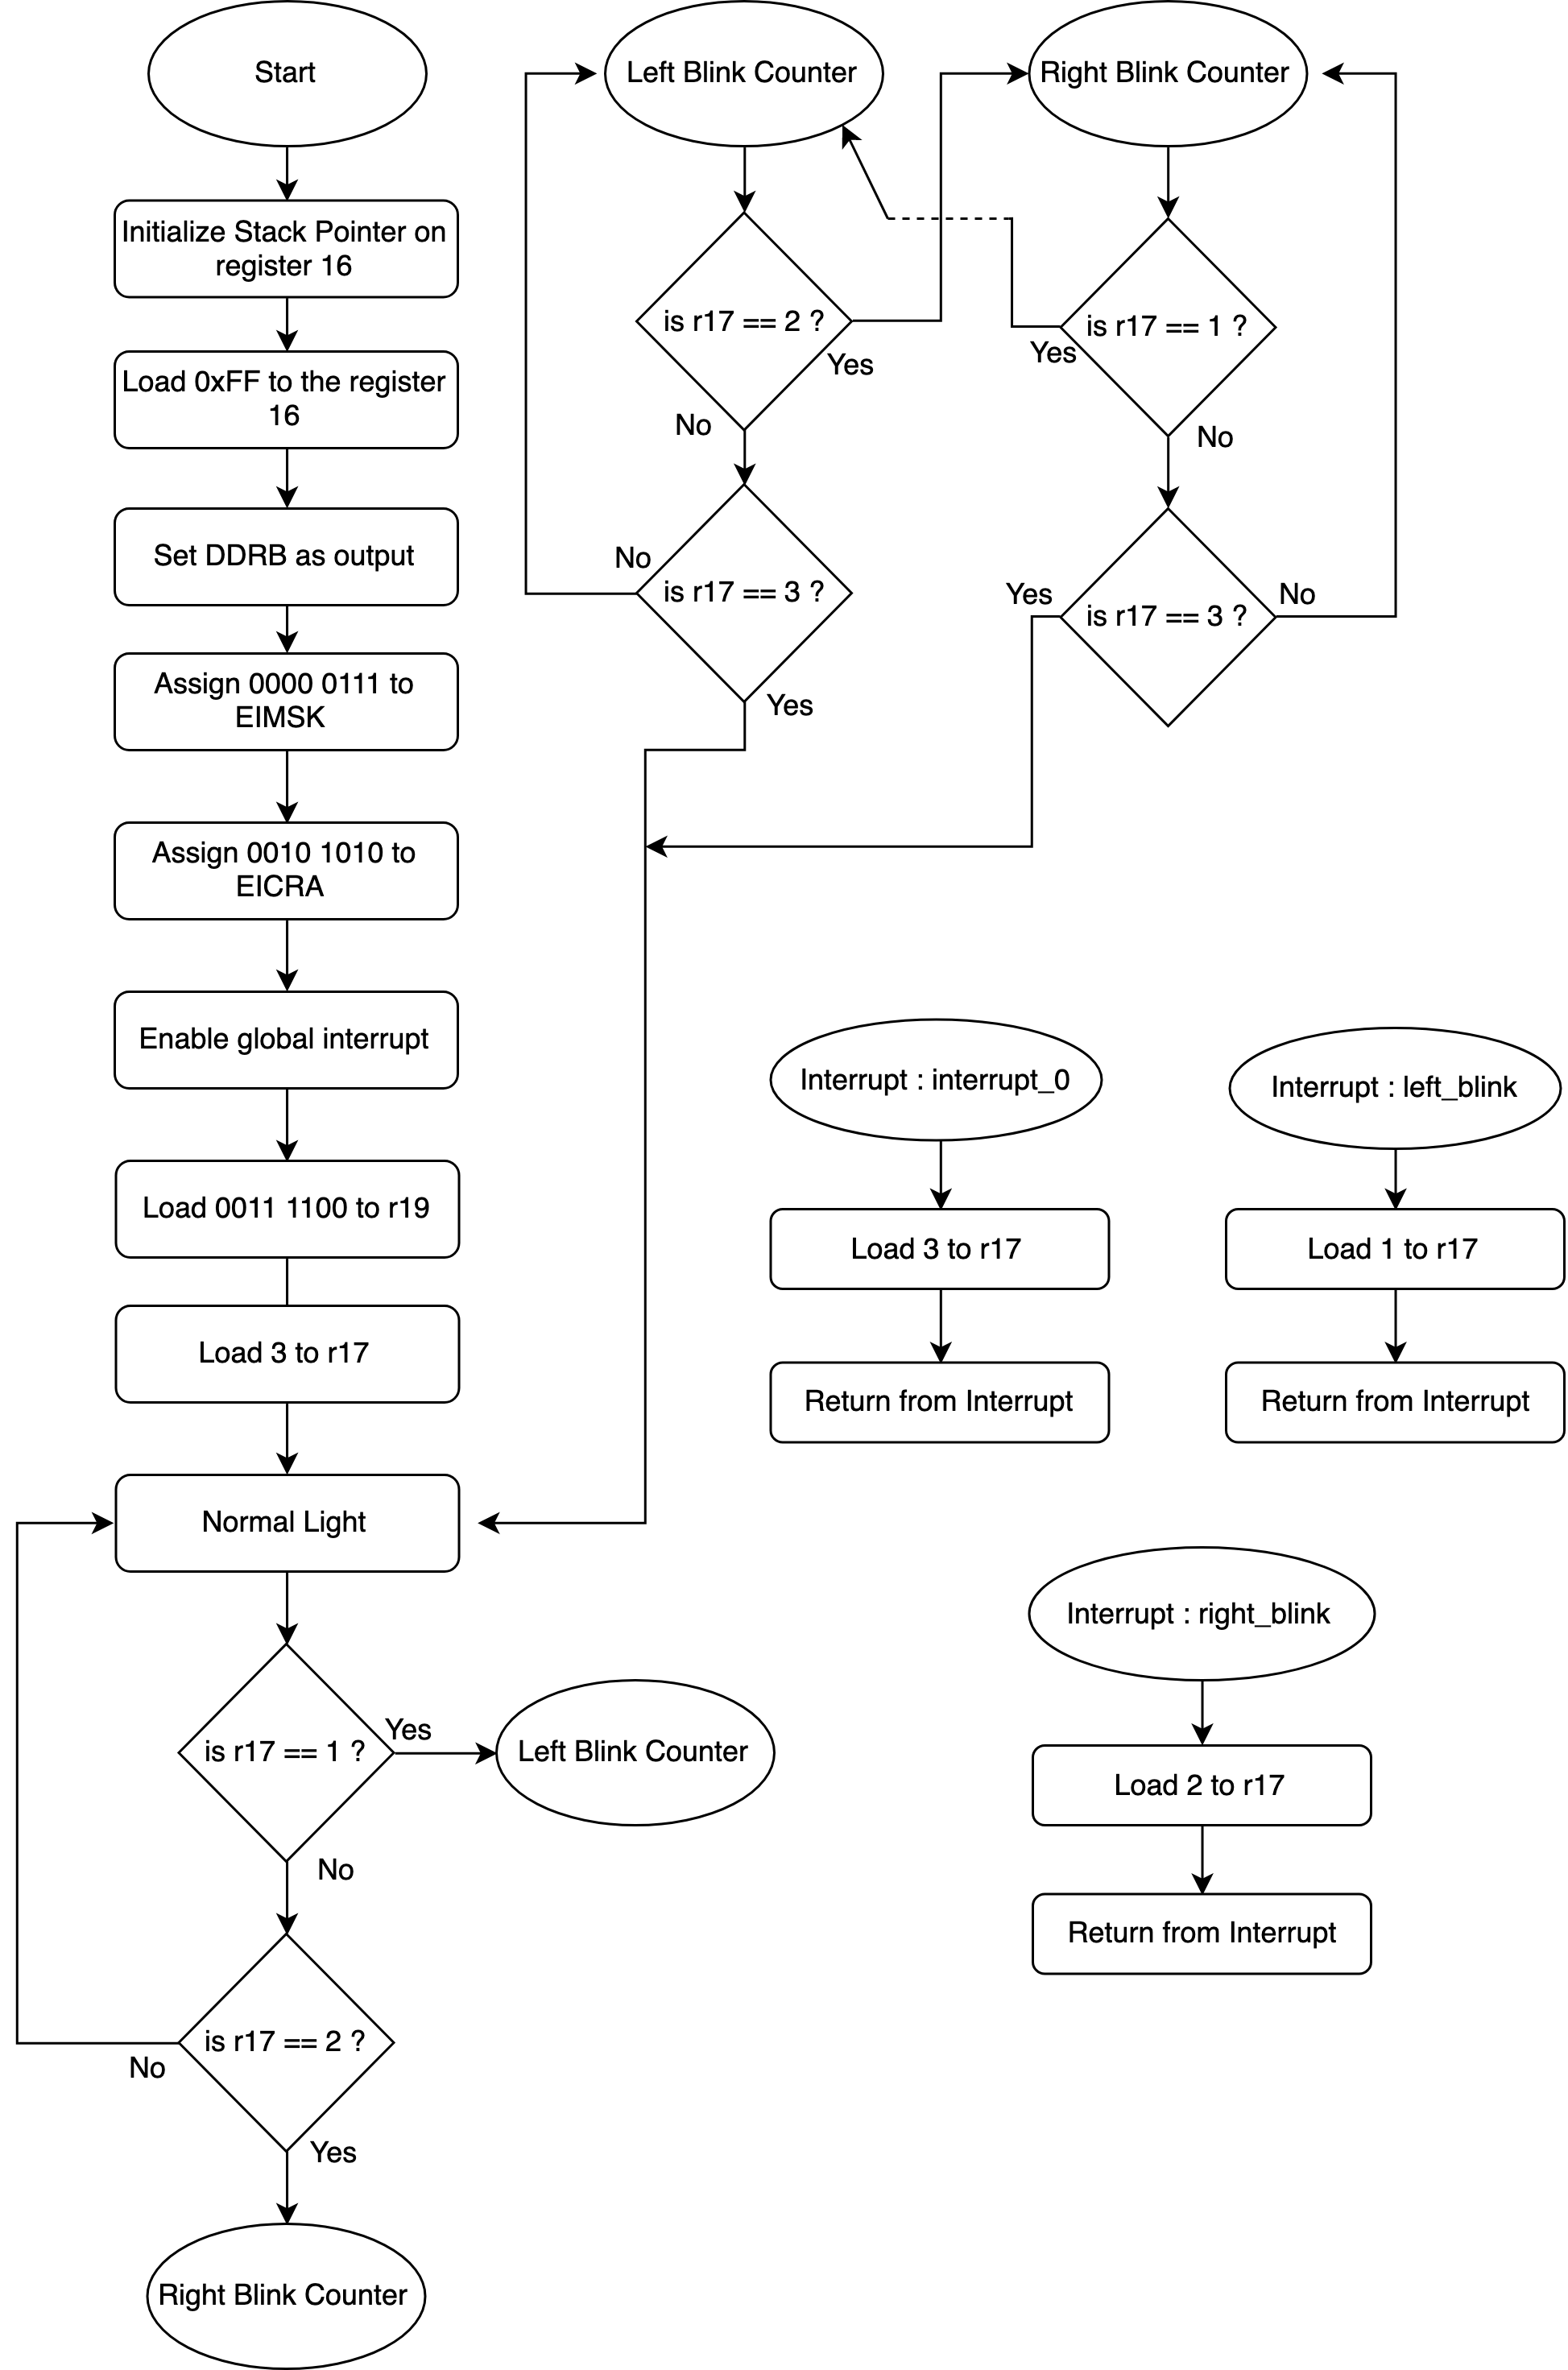
\includegraphics[width=\textwidth/2 ]{flowchart/task3_flowchart.png}
\end{center}
\caption{Task 3 flowchart}
\label{task3}
\end{figure}

\break

%TASK4
\section{Task 4}

\lstset{style=Asm}

\begin{lstlisting}
;>>>>>>>>>>>>>>>>>>>>>>>>>>>>>>>>>>>>>>>>>>>>>>>>>>>>>>>>>>>
; 1DT301, Computer Technology I
; Date: 2016-09-15
; Author:
;	Anas Kwefati
;
; Lab number: 3
; Title: Interrupts
;
; Hardware: STK600, CPU ATmega2560
;
; Function: We have to add the function for stop light. When braking, all LEDs
; are turned ON only when there is no right blink or left blink.
;	If there is RIGHT BLINK then :
; Turning Right and Brake -> LED 4 to 7 are ON and 0 to 3 are Blinking
; Turning Left and Brake -> LED 0 to 3 are ON and 4 to 7 are blinking
;
; Input ports: PORTD checks if we pressed the button
;
; Output ports: PORTB turns on/off the light (LEDs)
;
; Subroutines: If applicable.
; Included files: m2560def.inc
;
; Other information: Use INT2 for the Brake
;
; Changes in program: (Description and date)
;<<<<<<<<<<<<<<<<<<<<<<<<<<<<<<<<<<<<<<<<<<<<<<<<<<<<<<<<<<<
.include "m2560def.inc"
;The term VECTOR means nothing more than that each interrupt has its specific address where it jumps to.
; The term TABLE means it is a list of jump instructions. This is a list of rjmp or jmp instructions, sorted by interrupt priority

.org 0x00 ;This is the location that the program will start executing from
rjmp start

.org INT0addr
rjmp right_blink

.org INT1addr
rjmp left_blink

.org INT2addr
rjmp braking

.org INT3addr
rjmp normal

.org 0x72
start:
	; Initialize SP, Stack Pointer
	ldi r16, HIGH(RAMEND) ; R20 = high part of RAMEND address
	out SPH,r16 ; SPH = high part of RAMEND address
	ldi r16, low(RAMEND) ; R20 = low part of RAMEND address
	out SPL,r16 ; SPL = low part of RAMEND address



	;Main program initialization
	ldi r16, 0xFF ;
	out DDRB, r16 ; we set the DDRB as output

	ldi r29, 0x00
	out DDRD, r29


	ldi r17, 0b00001111 ;we set the corresponding bit number to enable the related interrupt here INT0
	out EIMSK, r17 ; Toggle external interrupt requests


	ldi r17, 0b10101010 ;We define the type of signals that activates the external interrupt , here we set it as falling edge to activate the interrupt
	sts EICRA, r17 ;we configure when to switch the external interrupt

	sei ;enabling all interrupts

	ldi r19,0b00111100 ;normal light

	ldi r27, 0b00000000 ;braking light

	ldi r26, 0b00000011 ;For SUB to turn on the correct light
	ldi r22, 0b11000000

	ldi r17, 4 ;To check what we pushed

main_program:

	cpi r17, 4 ;we compare r17 with 4
	breq normal_light ;if r17 is r17 == 4 then go to normal_light

rjmp main_program

normal_light :
	out PORTB, r19 ;Output 0b0011 1100 to PORTB

	;We compare to see what we have pressed

	cpi r17,1
	breq left_blink_counter

	cpi r17,2
	breq right_blink_counter

	cpi r17,3
	breq braking_light_normal

rjmp normal_light

braking_light_left:
	ldi r29, 0b11111111 ;we add 0b1111 1111 to r29
	;This one will check if we are still pressing any Switches or not
	;We want it to see that we don't press any switch
	in r28, PIND ;We take the data of PIND and put it in r28
	cp r28, r29 ;we compare r29 and r28
	breq left_blink_counter ;if r28==r29 we go to left_blink_counter

rjmp braking_light_left



braking_light_right:
;Same IDEA as braking_light_left
	ldi r29, 0b11111111

	in r28, PIND
	cp r28, r29
	breq right_blink_counter

rjmp braking_light_right

braking_light_normal:

	ldi r29, 0b11111111

	in r28, PIND
	cp r28, r29
	breq normal_light

rjmp braking_light_normal


left_blink_counter:
	ldi r18, 0b11101111

	;WE COMPARE
	cpi r17,2
	breq right_blink_counter



left_loop:
	mov r20,r18
	sub r20, r26
	out PORTB, r20 ;we put the value of r18 to PORTB which should turn on the light
	call Delay
	com r18
	LSL r18
	com r18


	;Check if everything is off if true then go to ring counter to make infinite loop
	ldi r24,0xFF
	cp r24, r18
	breq left_blink_counter

	;WE COMPARE
	cpi r17,2
	breq right_blink_counter

	;cpi r17,3
	;breq braking_light_left

	cpi r17, 4
	breq normal_light


rjmp left_loop

right_blink_counter:
	ldi r18, 0b11110111

	;WE COMPARE
	cpi r17,1
	breq left_blink_counter


right_loop:
	mov r25,r18
	sub r25, r22
	out PORTB, r25 ;we put the value of r18 to PORTB which should turn on the light

	call Delay
	com r18
	LSR r18
	com r18

	;Check if everything is off if true then go to ring counter to make infinite loop
	ldi r24,0xFF
	cp r24, r18
	breq right_blink_counter

	;WE COMPARE
	cpi r17,1
	breq left_blink_counter

	;cpi r17,3
	;breq braking_light

	cpi r17,4
	breq normal_light

rjmp right_loop


;INTERRUPS

left_blink: ;LEFT BLINK
	ldi r17, 1
	ldi r26, 0b00000011 ;For SUB to turn on the correct light
reti

right_blink: ;RIGHT_BLINK
	ldi r17,2
	ldi r22, 0b11000000 ;We use it for SUB and to reset r22
reti

braking: ;BRAKING
	ldi r17, 3
	out PORTB, r27 ;Turn on r27

	cpi r17,1 ;if we pressed 1 (left) we go to change_1
	breq change_1

	cpi r17,2
	breq change_2

	change_1:
		ldi r26, 0b00001111 ;For SUB to turn on the correct light for braking

	change_2 :
		ldi r22, 0b11110000


reti

normal :
	ldi r17, 4
	out PORTB, r19
reti

Delay :
; Generated by delay loop calculator
; at http://www.bretmulvey.com/avrdelay.html

	ldi  r21, 5
    ldi  r23, 20
    ldi  r24, 175
L1: dec  r24
    brne L1
    dec  r23
    brne L1
    dec  r21
    brne L1
	ret

\end{lstlisting}
\break
\begin{figure}
\begin{center}
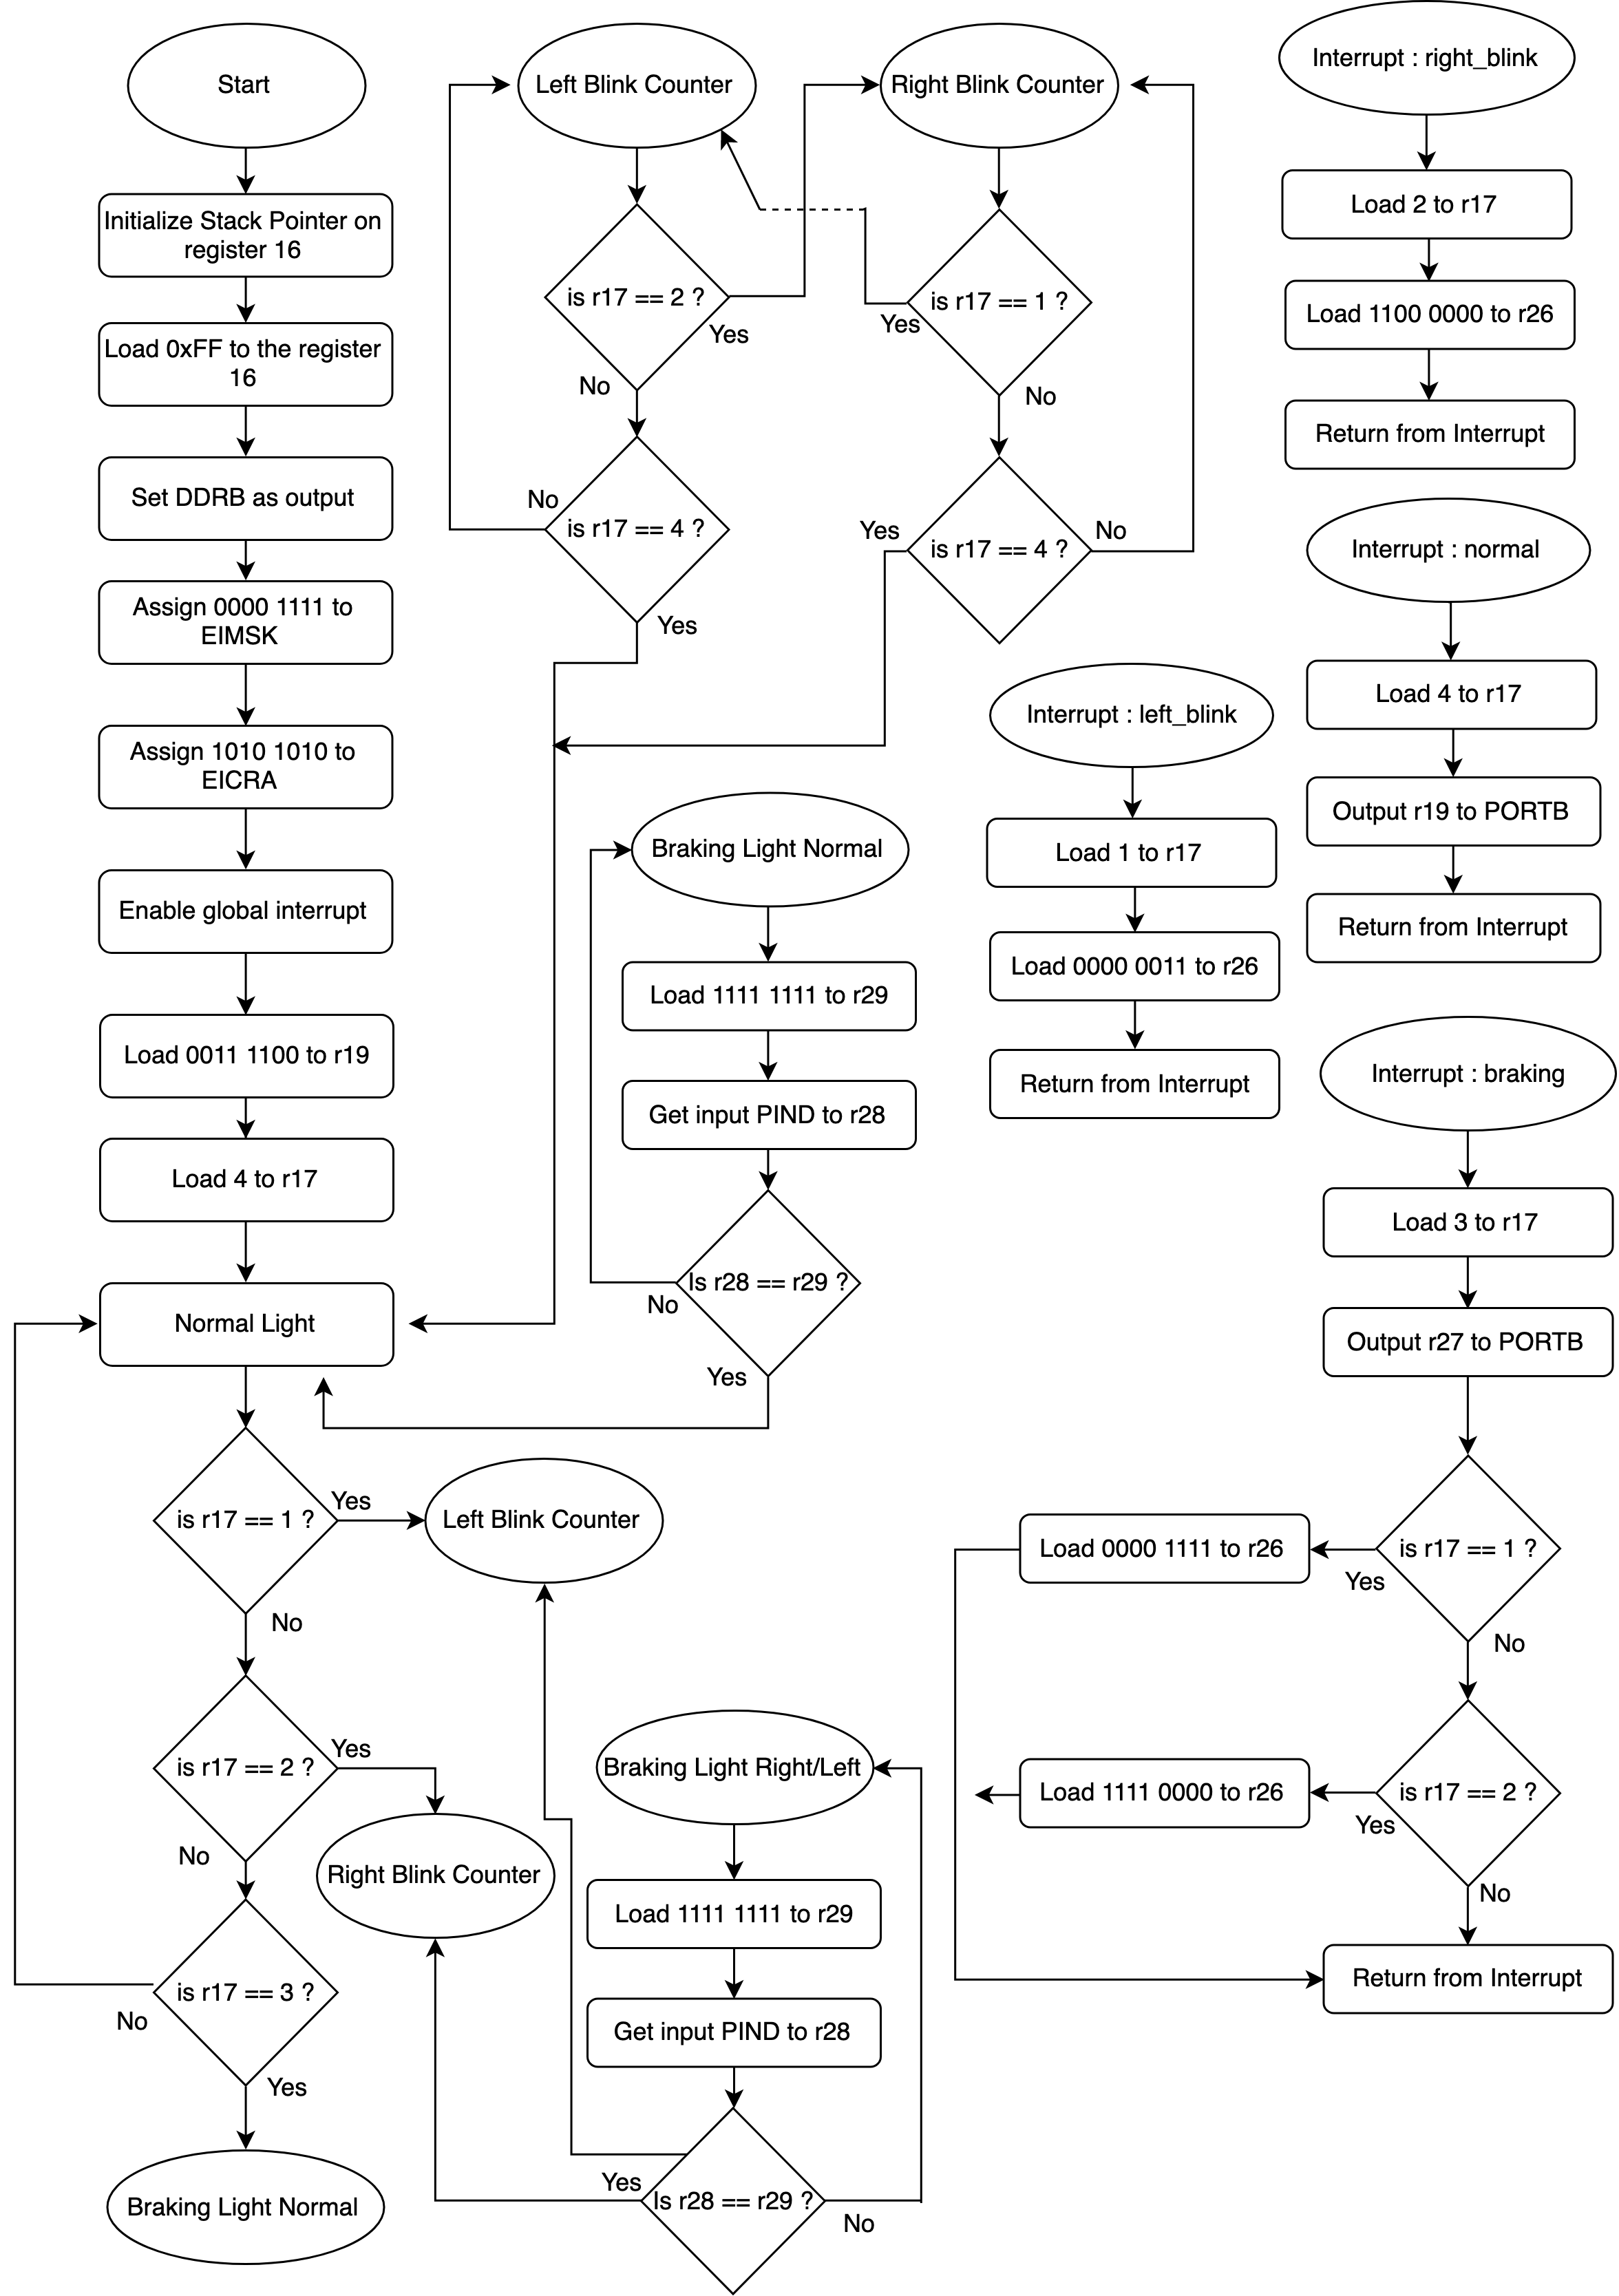
\includegraphics[width=\textwidth/1 ]{flowchart/task4_flowchart.png}
\end{center}
\caption{Task 4 flowchart}
\label{task4}
\end{figure}

\break 

% Prints your bibliography database xxx.bib
\bibliographystyle{IEEEtran}
\bibliography{ref.bib}

\end{document}
